\documentclass[12pt,letterpaper, onecolumn]{exam}
\usepackage{amsmath}
\usepackage{amssymb}
\usepackage{xcolor}
\usepackage{graphicx}
\usepackage{placeins}
\usepackage[lmargin=71pt, tmargin=1.2in]{geometry}  %For centering solution box
% \chead{\hline} % Un-comment to draw line below header
\thispagestyle{empty}   %For removing header/footer from page 1

\begin{document}

\begingroup  
    \centering
    \LARGE AE 370\\
    \LARGE Project 1 (Group)\\[0.5em]
    \large April 11, 2025\\[0.5em]
    \large Nick Djordjevic, Zhiwei Jiang, Anush Rajan, Aadyanth Rao, Ella Greer\par
\endgroup
\rule{\textwidth}{0.4pt}
\pointsdroppedatright   %Self-explanatory
\printanswers
\renewcommand{\solutiontitle}{\noindent\textbf{Ans:}\enspace}   %Replace "Ans:" with starting keyword in solution box

% google colab link (delete for final submission): https://colab.research.google.com/drive/1ye39sIHo21pxyWUGkeYKWmL4dgVNpXMs#scrollTo=bEBGcQKsQeBT

\section{Introduction}

Landing gear plays a critical role in aerospace engineering, ensuring a smooth and controlled touchdown. The shock absorption capabilities of the landing gear affect passenger comfort, structural integrity, and aircraft performance. 

The landing gear of an aircraft can be modeled as a mass-spring-damper system. The shock absorber, modeled by a damper and spring, connects the aircraft body and wheel. Both the aircraft body and wheel are assumed to be rigid and modeled as masses. The model of this system also considers the frictional force that occurs at the contact point of the wheel and the ground to simulate real-world conditions. 

This project explores the coupled mass-spring-damper dynamics of landing gear during touchdown, focusing on how damping influences touchdown loads and whether an optimal stiffness-damping ratio exists for smooth landings.

\subsection{Objective}
The primary goal of this study is to:
\begin{itemize}
    \item Develop a mathematical model for a coupled mass-spring-damper system representing landing gear dynamics.
    \item Implement a numerical method to simulate the system’s response under various conditions.
    \item Analyze the effects of damping and stiffness on landing impact forces.
\end{itemize}

\subsection{Organization}
This document will be organized by enumerated parts in the content section as listed in the report guidelines. A brief overview of the structure is as follows:

\begin{itemize}
\item Part 1: Present a dynamical system that is relevant to engineering.
\item Part 2: Present a numerical method that is appropriate to study the questions that you've asked of the dynamical system.
\item Part 3: Demonstrate correct implementation of the method.
\item Part 4: Present results that meaningfully address the question you ask.
\item Part 5: A summary description of everyone's roles in the project.
\item Part 6: Appendix
\end{itemize}

\section{Content}
\begin{questions}

    \question[22 Points] Present a dynamical system that is relevant to engineering. \droppoints

        \begin{parts}
            \part Describe why that dynamical system is interesting / important to understand

            \part Synthesize a question or set of questions that you want to ask of that dynamical system

            \part Convey your dynamical system mathematically. Be sure that you specify any parameters that the dynamical system depends on and which parameter value ranges are relevant to the specific questions you want to explore.
        \end{parts}

        \begin{solution}
            \begin{parts}
                \part \textbf{Significance and Applications of the Coupled Mass-Spring-Damper System for Landing Gear Shock Absorption:}

                \vspace{5mm}

                The study of the coupled mass-spring-damper system in landing gear shock absorption is essential for understanding the dynamic response of aircraft during landing. This system models how energy is dissipated upon touchdown and how forces are transmitted through the landing gear to the aircraft structure. By analyzing this system, engineers can design landing gear that minimizes impact forces, enhances passenger comfort, and extends the lifespan of aircraft components.

                \vspace{5mm}

                \textbf{Engineering Significance and Applications:}

                \vspace{5mm}

                In aerospace engineering, the structural integrity of an aircraft is paramount. During landing, the aircraft experiences significant dynamic loads, which can introduce high stress concentrations in the fuselage, wings, and undercarriage. The mass-spring-damper system helps mitigate these effects by absorbing and dissipating energy, preventing excessive deformation and fatigue damage. 

Key considerations include:
\begin{itemize}
    \item Reducing impact forces transmitted to the airframe, minimizing structural fatigue.
    \item Enhancing the lifespan of aircraft components by controlling vibrational loads.
    \item Distributing landing loads effectively to avoid localized stress failures.
\end{itemize}

\textit{Applications to Landing Gear Design}

The landing gear is one of the most critical components of an aircraft, directly responsible for handling impact forces upon touchdown. The mass-spring-damper system is fundamental to landing gear design, where its primary function is to absorb kinetic energy and provide a controlled deceleration of the aircraft.

Key design applications include:
\begin{itemize}
    \item \textbf{Shock Absorption:} The spring stores potential energy, while the damper dissipates energy as heat, allowing for a smooth landing.
    \item \textbf{Ground Friction and Stability:} The interaction between the wheel and the ground ensures controlled rolling motion, preventing skidding while maintaining traction.
    \item \textbf{Landing Performance Optimization:} Engineers analyze the spring stiffness and damping characteristics to achieve optimal energy dissipation and minimize bounce after touchdown.
    \item \textbf{Adaptability to Different Aircraft Weights:} The design can be adjusted for varying aircraft weights, from small private planes to large commercial airliners, ensuring stability under different loading conditions.
\end{itemize}

\textit{Applications to Vibration Control}

Beyond landing gear design, mass-spring-damper systems are widely used in aerospace for vibration control. These systems help manage oscillatory forces that arise during aircraft operations, including turbulence, taxiing, and takeoff.

Key applications include:
\begin{itemize}
    \item \textbf{Damping Unwanted Vibrations:} The landing gear must mitigate vibrations that arise from ground contact, ensuring comfort and preventing excessive wear on components.
    \item \textbf{Resonance Avoidance:} Proper tuning of the system ensures that natural frequencies do not coincide with external excitations, preventing destructive resonant conditions.
    \item \textbf{Noise Reduction:} Effective vibration control helps reduce noise levels inside the aircraft cabin, improving passenger experience.
\end{itemize}

\vspace{5mm}

                \textbf{Uniqueness and Key Properties of the System:}

                \vspace{5mm}
                    This system is particularly unique due to its coupled nature and the presence of translational and rotational dynamics. Several properties make it a valuable subject of analysis:
                        \begin{itemize}
                            \item \textit{Coupled Dynamics:} Unlike simple single-degree-of-freedom (SDOF) models, this system involves interactions between vertical displacement, wheel rotation, and horizontal motion.
                            \item \textit{Energy Dissipation:} The damper plays a critical role in dissipating kinetic energy, reducing rebound effects, and preventing excessive oscillations after landing.
                            \item \textit{No-Slip Condition:} The rolling constraint introduces additional complexity, enforcing a kinematic relationship between the translational and rotational motion of the wheel.
                            \item \textit{Frictional Effects:} The presence of friction at the tire-ground interface influences the overall dynamics and stability of the system, impacting real-world performance.
                            \item \textit{Nonlinearities and External Forces:} Real-world applications may introduce nonlinear damping, varying stiffness, and external disturbances such as crosswinds or runway imperfections, making the system behavior more intricate and interesting to analyze.
                        \end{itemize}

                \part This project aims to answer the following questions:
                    \begin{itemize}
                        \item Can we optimize the stiffness/damping ratio for smooth landings?
                        \item How do changes in damping affect touchdown loads?
                    \end{itemize}

                \part 
                
                
        \textbf{Free Body Diagram:}\\
        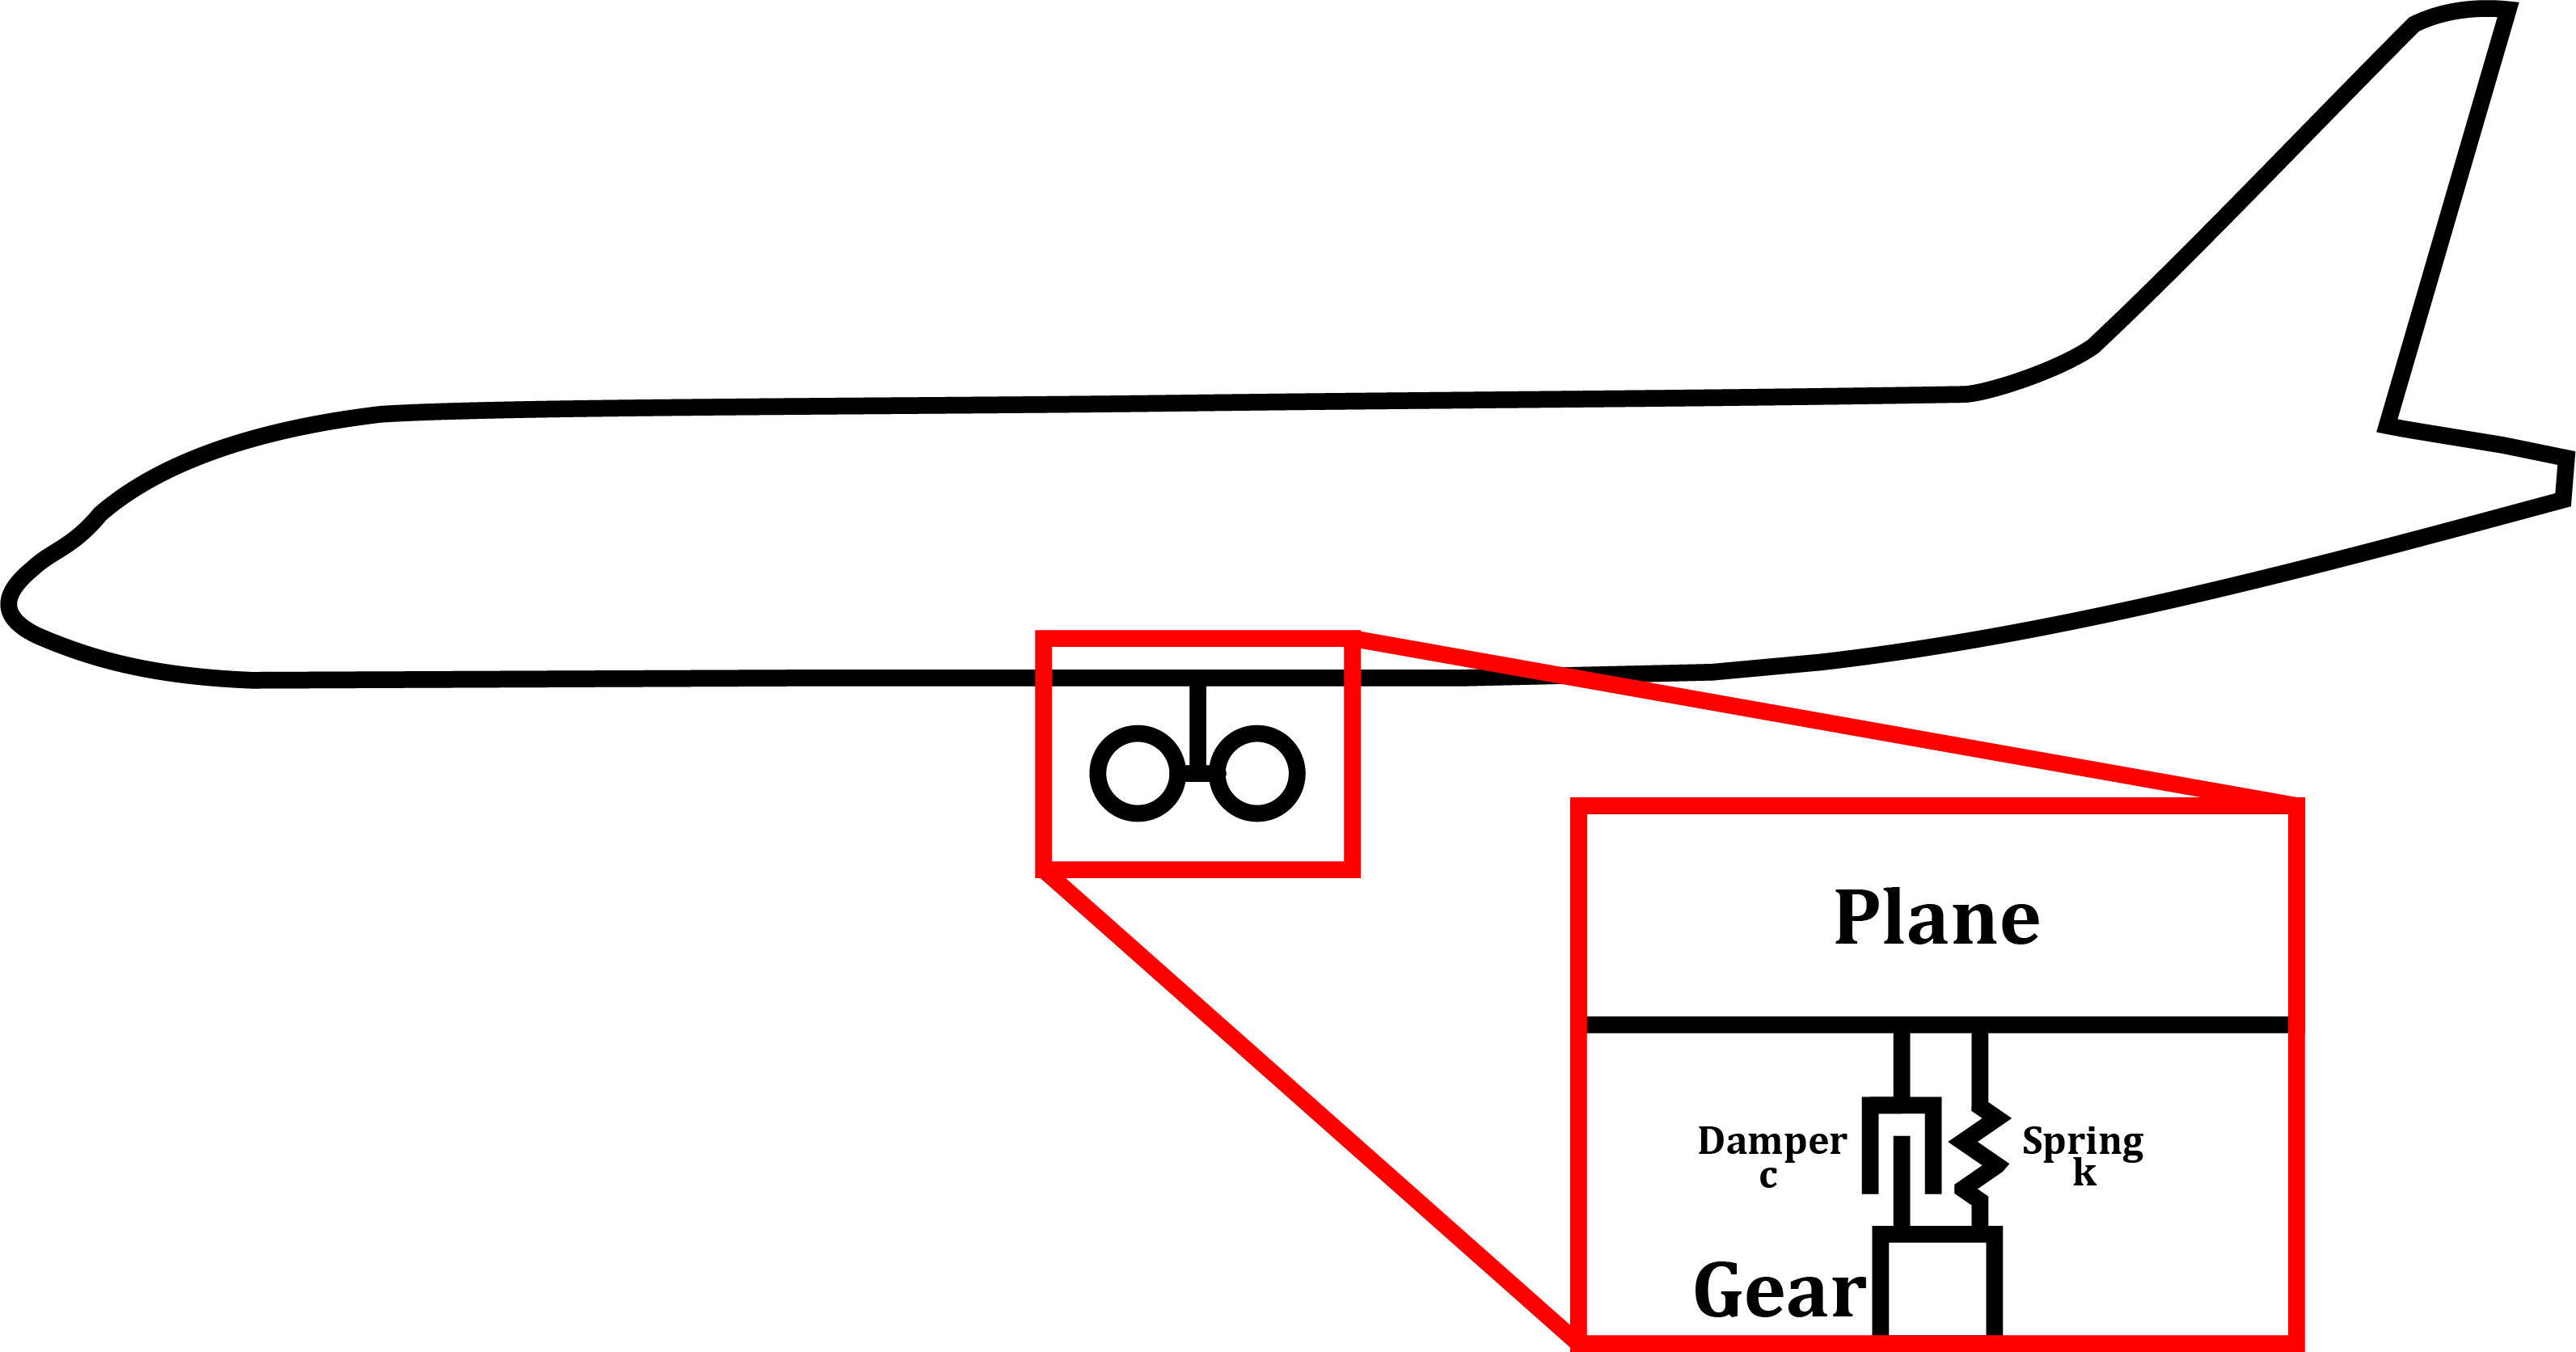
\includegraphics[scale = 0.5]{FBD.png}
        
        \textbf{System Parameters:}

        \begin{itemize}
            \item $m$ : Mass of the aircraft section associated with the landing gear
            \item $k$ : Stiffness of the spring
            \item $c$ : Damping coefficient of the damper
            \item $z$ : Vertical displacement of the mass (measured from equilibrium)
            \item $z_g$ : Vertical displacement of the ground (if uneven terrain is considered)
            \item $N$ : Normal force exerted by the ground on the wheel
            \item $F_f$ : Friction force at the wheel-ground contact point
            \item $I_w$ : Moment of inertia of the wheel
            \item $r$ : Radius of the wheel
            \item $\theta$ : Angular displacement of the wheel
            \item $\mu$ : Coefficient of friction between the wheel and the ground
        \end{itemize}

        \textbf{Assumptions}
            \begin{enumerate}
                \item The aircraft mass moves only in the vertical direction.
                \item The wheel is treated as a rigid body.
                \item The system is modeled in 2D with forces acting in the vertical and horizontal directions.
                \item \textbf{No-slip condition} implies a kinematic constraint between wheel rotation and translational motion.
            \end{enumerate}

        \textbf{First Order Equations of Motion:}

        \vspace{5mm}
            \textit{Vertical Motion of the Aircraft Mass:}
                Applying Newton’s Second Law to the aircraft mass:
        \begin{equation}
            m\ddot{z} = -k(z - z_g) - c(\dot{z} - \dot{z}_g) + N - mg
        \end{equation}

        \textit{Vertical Force Balance on the Wheel:}
    \begin{equation}
        N = mg - k(z - z_g) - c(\dot{z} - \dot{z}_g)
    \end{equation}

        \textit{Horizontal Motion of the Wheel:}
            Newton’s Second Law in the horizontal direction:
    \begin{equation}
    m_w \ddot{x} = F_f
    \end{equation}
    where $m_w$ is the mass of the wheel.

    \textit{Rotational Motion of the Wheel:}
    Using torque balance about the wheel’s center:
    \begin{equation}
    I_w \ddot{\theta} = -r F_f
    \end{equation}

    \textit{No-Slip Condition:}
    Since the wheel rolls without slipping:
    \begin{equation}
    \dot{x} = r \dot{\theta}
    \end{equation}
    Differentiating:
    \begin{equation}
    \ddot{x} = r \ddot{\theta}
    \end{equation}
    Substituting into the rotational equation:
    \begin{equation}
    I_w \frac{\ddot{x}}{r} = -r F_f
    \end{equation}

    \textit{Expressing Friction Force:}
    Solving for $F_f$:
    \begin{equation}
    F_f = -\frac{I_w}{r^2} \ddot{x}
    \end{equation}

    Substituting into the horizontal motion equation:
    \begin{equation}
    m_w \ddot{x} = -\frac{I_w}{r^2} \ddot{x}
    \end{equation}

    Rearranging:
    \begin{equation}
    \left( m_w + \frac{I_w}{r^2} \right) \ddot{x} = 0
    \end{equation}

    \textbf{Second Order Form of the Equations of Motion}:

    \vspace{5mm}
    The system's equations of motion can be written as:
    \begin{align}
    m\ddot{z} + c(\dot{z} - \dot{z}_g) + k(z - z_g) &= N - mg \\
    N &= mg - k(z - z_g) - c(\dot{z} - \dot{z}_g) \\
    \left( m_w + \frac{I_w}{r^2} \right) \ddot{x} &= 0
    \end{align}

    \section*{First-Order Form of the Equations of Motion}
    
To convert this into a first-order system, we define the state variables:

\begin{equation}
    x_1 = z, \quad x_2 = \dot{z}, \quad x_3 = x, \quad x_4 = \dot{x}.
\end{equation}

\pagebreak

Taking their time derivatives:

\begin{equation}
    \dot{x}_1 = x_2, \quad \dot{x}_3 = x_4.
\end{equation}

Solving for \( \ddot{z} \) using the first equation:

\begin{equation}
    \ddot{z} = \frac{N - mg - c(x_2 - \dot{z}_g) - k(x_1 - z_g)}{m}.
\end{equation}

Substituting \( N \) from the second equation:

\begin{equation}
    \ddot{z} = \frac{mg - k(x_1 - z_g) - c(x_2 - \dot{z}_g) - mg - c(x_2 - \dot{z}_g) - k(x_1 - z_g)}{m}.
\end{equation}

Simplifying:

\begin{equation}
    \ddot{z} = -\frac{2k(x_1 - z_g) + 2c(x_2 - \dot{z}_g)}{m}.
\end{equation}

For \( \ddot{x} \), from the third equation:

\begin{equation}
    \ddot{x} = 0.
\end{equation}



Thus, the first-order system is:

\begin{align}
    \dot{x}_1 &= x_2, \\
    \dot{x}_2 &= -\frac{2k(x_1 - z_g) + 2c(x_2 - \dot{z}_g)}{m}, \\
    \dot{x}_3 &= x_4, \\
    \dot{x}_4 &= 0.
\end{align}

\pagebreak
    \textbf{How the EOMs answer the Questions Outlined in Part (b):}  

    \vspace{5mm}
    The normal force equation shows that the peak reaction force \( N \) is influenced by the damping coefficient \( c \). If \( c \) is too low, the system exhibits excessive oscillations, leading to multiple impacts and higher effective touchdown loads. Conversely, if \( c \) is too high, the system dissipates energy too rapidly, increasing the peak impact force transmitted to the airframe. The optimal damping ratio minimizes the peak touchdown loads while ensuring energy dissipation occurs in a controlled manner.

    \vspace{5mm}
    
    A smooth landing is characterized by minimal bouncing and a rapid transition to a steady state. From the vertical motion equation, the damping term \( c(\dot{z} - \dot{z}_g) \) determines how quickly oscillations decay. By optimizing \( c \), engineers can achieve critical or slightly overdamped behavior, which prevents excessive bouncing and ensures a stable landing. If \( c \) is underdamped, the system oscillates excessively, increasing the likelihood of an unstable landing. If \( c \) is overdamped, energy dissipation is too slow, which may prolong the landing process. Therefore, the probability of a smooth landing is maximized when damping is tuned to minimize residual oscillations without increasing peak loads.

            \end{parts}
        \end{solution}


    \question[22 Points] Present a numerical method that is appropriate to study the questions that you’ve asked of the dynamical system. \droppoints

        \begin{parts}
            \part Justification for why the method is appropriate to address the questions you want to probe in your dynamical system, using accuracy, stability, and cost consideration

            \part Mathematical derivation of the method including its error and stability properties

            \part Algorithmic summary of how the method advances a solution from some time instance $t_k$ to $t_{k+1}$
        \end{parts}

        \begin{solution}
        
            \begin{parts}
            
                \part \textbf{RK4 Method for the Coupled Mass-Spring-Damper System}

The fourth-order Runge-Kutta (RK4) method is a widely used explicit, one-step numerical integration technique for solving systems of first-order ordinary differential equations (ODEs). Given that the equations of motion for the Coupled Mass-Spring-Damper for Landing Gear Shock Absorption system have been converted into first-order form, RK4 is a highly appropriate method for simulating the dynamics of this system. Below, we outline why this method is suitable in terms of its accuracy, stability, computational cost, and ability to answer key engineering questions.

\subsubsection*{Method Classification}
\begin{itemize}
    \item \textbf{Type:} One-step method
    \item \textbf{Nature:} Explicit
    \item \textbf{Applicable Form:} First-order systems of ODEs
\end{itemize}

\subsubsection*{Why an Explicit, One-Step Method is the Best Choice for This System}

\textit{Explicit Method:} The RK4 method is explicit, meaning that each new step in the solution is computed using only known values from the previous step, without requiring the solution of a system of algebraic equations. This makes it computationally efficient and avoids the complexity of solving nonlinear implicit equations at each step. 

For this system:
\begin{itemize}
    \item The equations of motion are not highly stiff under normal operating conditions, meaning an explicit method remains stable for reasonable time step sizes.
    \item Explicit methods like RK4 allow for direct evaluation of velocity and force responses, which are crucial in understanding landing gear shock absorption performance.
    \item Implicit methods such as Newmark-Beta would require iterative solvers, increasing computational cost unnecessarily for a system that does not demand unconditional stability.
\end{itemize}

\subsubsection*{Accuracy Considerations}

Since RK4 is a one-step method, it does not rely on previous time steps beyond the immediately preceding step. This provides several advantages:
\begin{itemize}
    \item One-step methods are better suited for handling abrupt changes in force (e.g., touchdown impact) because they do not require past solutions, which might introduce lag in response.
    \item Multi-step methods such as Adams-Bashforth may require special initialization and can accumulate numerical errors from previous steps, which could be problematic when analyzing short-duration, high-impact events.
    \item A one-step approach is more flexible in adaptive time stepping, which is useful if refinement is needed near touchdown.
\end{itemize}

The local truncation error (LTE) is the error made in a single step of the method, assuming perfect knowledge of the solution at the previous time step. For a one-step method like RK4, the LTE is given by:
\[
\tau_k = y(t_{k+1}) - \Phi(t_k, y_k, \Delta t)
\]
where \( \Phi \) is the RK4 update formula and \( y(t_{k+1}) \) is the exact solution. For RK4, it can be shown that:
\[
\tau_k = \mathcal{O}(\Delta t^5)
\]
This implies that the local error per step decreases proportionally to \( \Delta t^5 \) as the step size \( \Delta t \) becomes smaller.

The global truncation error (GTE) is the cumulative effect of local truncation errors over all steps. Since there are approximately \( \frac{T}{\Delta t} \) steps in an interval \( [0, T] \), and each contributes an \( \mathcal{O}(\Delta t^5) \) error, the total accumulated error is:
\[
\text{Global Error} = \mathcal{O}(\Delta t^4)
\]

This makes RK4 a fourth-order accurate method globally, meaning the global error decreases rapidly with smaller time steps, making it well-suited for high-precision simulations. RK4's level of accuracy is significantly higher than that of simpler methods such as Forward Euler (\( \mathcal{O}(\Delta t) \)) or Heun’s method (\( \mathcal{O}(\Delta t^2) \)), making it highly effective in capturing the detailed dynamics of the system, including transient behaviors and impact responses. This level of accuracy ensures reliable simulations for engineering analysis and design.

\textit{More information about the error of this numerical method is provided in part (b)}

\subsubsection*{Stability Considerations}

The general solution to a linear differential equation is:
\[
u_j(t) = \exp\left[\lambda_j(t - t_0)\right](u_0)_j
\]
For numerical stability, we examine the behavior of the RK4 method under this form. The RK4 method is stable when:
\[
|R(z)| \leq 1, \quad \text{where } R(z) = 1 + z + \frac{z^2}{2!} + \frac{z^3}{3!} + \frac{z^4}{4!}, \quad z = \lambda \Delta t
\]
RK4 is conditionally stable and not astable. Its absolute stability region approximately includes values where \( \text{Re}(z) < 0 \) and \( |z| \lesssim 2.8 \). For systems with large damping or stiffness (i.e., stiff systems), RK4 may require small time steps to maintain stability. However, for moderately stiff or well-scaled systems, RK4 remains stable and effective.

\subsubsection*{Cost and Implementation Considerations}

RK4 requires four evaluations of the right-hand side function \( \mathbf{f}(t, \mathbf{x}) \) per time step. Despite this moderate computational cost, it avoids matrix inversions and nonlinear solvers, making it straightforward to implement in numerical computing environments such as Python or MATLAB. Its simplicity and reliability make it a practical choice for time-domain simulations.

\subsubsection*{Relevance to Engineering Questions}

The RK4 method is highly suitable for addressing the two core engineering questions:

\begin{enumerate}
    \item \textbf{Can we optimize the stiffness/damping ratio for smooth landings?} \\
    The RK4 method accurately tracks the system’s response, allowing engineers to test different values of stiffness \( k \) and damping \( c \) to evaluate their effect on the smoothness of touchdown. A smooth landing is characterized by:
    \begin{itemize}
        \item A minimal spike in acceleration \( \ddot{z} \), reducing impact forces.
        \item A fast but well-damped return to equilibrium, preventing excessive oscillations.
        \item Low overshoot and minimal rebound, which improves passenger comfort and structural longevity.
    \end{itemize}
    By running simulations with RK4, engineers can systematically adjust damping and stiffness to find an optimal combination that minimizes peak accelerations and excessive oscillations.

    \item \textbf{How do changes in damping affect touchdown loads?} \\
    The normal force \( N \), which affects structural loads during landing, is given by:
    \[
    N = mg - k(z - z_g) - c(\dot{z} - \dot{z}_g)
    \]
    The RK4 method allows precise evaluation of how \( N \) varies over time for different damping values \( c \). Specifically:
    \begin{itemize}
        \item Insufficient damping results in high peak loads due to excessive oscillations.
        \item Overdamping increases the duration of load application, which may lead to inefficient energy dissipation.
        \item Critically or optimally damped cases provide the best balance, reducing peak forces while ensuring a smooth energy dissipation profile.
    \end{itemize}
    By analyzing simulated normal force profiles with RK4, engineers can determine how damping affects the probability of a smooth landing. A well-optimized damping coefficient increases the probability of a successful landing by minimizing peak force fluctuations while maintaining adequate shock absorption.
\end{enumerate}



\part \textbf{Mathematical Derivation of the RK4 Method Including Error and Stability Properties}

The classical fourth-order Runge-Kutta (RK4) method is designed to solve initial value problems of the form:
\[
\frac{d\mathbf{x}}{dt} = \mathbf{f}(t, \mathbf{x}), \quad \mathbf{x}(t_0) = \mathbf{x}_0
\]
The RK4 method updates the solution from time \( t_k \) to \( t_{k+1} = t_k + \Delta t \) as follows:
\begin{align*}
k_1 &= \mathbf{f}(t_k, \mathbf{x}_k) \\
k_2 &= \mathbf{f}\left(t_k + \frac{\Delta t}{2}, \mathbf{x}_k + \frac{\Delta t}{2} k_1\right) \\
k_3 &= \mathbf{f}\left(t_k + \frac{\Delta t}{2}, \mathbf{x}_k + \frac{\Delta t}{2} k_2\right) \\
k_4 &= \mathbf{f}(t_k + \Delta t, \mathbf{x}_k + \Delta t k_3) \\
\mathbf{x}_{k+1} &= \mathbf{x}_k + \frac{\Delta t}{6}(k_1 + 2k_2 + 2k_3 + k_4)
\end{align*}

\textbf{Local Truncation Error (LTE):} The RK4 method has a local truncation error of order \( \mathcal{O}(\Delta t^5) \), which quantifies the error made in a single time step assuming the previous solution is exact:
\[
\tau_k = \mathbf{x}(t_{k+1}) - \mathbf{x}_{k+1} = \mathcal{O}(\Delta t^5)
\]

\textbf{Global Truncation Error (GTE):} Over multiple steps, the accumulated error grows proportionally to \( \mathcal{O}(\Delta t^4) \), making RK4 a globally fourth-order accurate method:
\[
\text{GTE} = \mathcal{O}(\Delta t^4)
\]

\textbf{Stability Properties:} For linear test equations of the form \( \frac{du}{dt} = \lambda u \), the stability function of RK4 is given by:
\[
R(z) = 1 + z + \frac{z^2}{2!} + \frac{z^3}{3!} + \frac{z^4}{4!}, \quad z = \lambda \Delta t
\]
The method is stable for values of \( z \) such that \( |R(z)| \leq 1 \). The absolute stability region includes much of the left half of the complex plane but does not include the entire negative real axis, meaning RK4 is not A-stable. Nonetheless, for non-stiff systems or systems where stiffness is moderate and time steps are chosen appropriately, RK4 remains stable and effective.

\part \textbf{Algorithmic Summary of RK4 Method}

The following is a step-by-step summary of how the RK4 method advances the solution from time \( t_k \) to \( t_{k+1} = t_k + \Delta t \):

\begin{enumerate}
    \item \textbf{Input:} Current time \( t_k \), current state \( \mathbf{x}_k \), time step \( \Delta t \), and function \( \mathbf{f}(t, \mathbf{x}) \)
    
    \item \textbf{Compute Slopes:}
    \begin{align*}
    k_1 &= \mathbf{f}(t_k, \mathbf{x}_k) \\
    k_2 &= \mathbf{f}\left(t_k + \frac{\Delta t}{2}, \mathbf{x}_k + \frac{\Delta t}{2} k_1\right) \\
    k_3 &= \mathbf{f}\left(t_k + \frac{\Delta t}{2}, \mathbf{x}_k + \frac{\Delta t}{2} k_2\right) \\
    k_4 &= \mathbf{f}(t_k + \Delta t, \mathbf{x}_k + \Delta t k_3)
    \end{align*}

    \item \textbf{Update State:}
    \[
    \mathbf{x}_{k+1} = \mathbf{x}_k + \frac{\Delta t}{6}(k_1 + 2k_2 + 2k_3 + k_4)
    \]

    \item \textbf{Advance Time:}
    \[
    t_{k+1} = t_k + \Delta t
    \]

    \item \textbf{Repeat:} Continue steps 2–4 until the final simulation time is reached.
\end{enumerate}

This algorithm is simple to implement and provides a reliable and accurate approach for integrating the coupled mass-spring-damper system. It is well-suited to probing design-related questions about stiffness and damping tuning in aircraft landing gear systems.

            
            \end{parts}
            
        \end{solution}

\question[22 Points] Demonstrate correct implementation of the method. This demonstration should include: \droppoints

\begin{parts}
    \part Appropriate error convergence studies that shows your method scales at the expected convergence rate

    \part An evaluation of which simulation parameters (e.g., time step size) your method needs to use so that you can accurately study the problem of interest
\end{parts}

\begin{solution}

    \begin{parts}

        \part 
        To rigorously confirm the correct implementation of our chosen numerical method—classical fourth-order Runge-Kutta (RK4)—we performed a detailed error convergence study. This process evaluates whether the global error scales with the theoretical convergence rate of the method, which is a critical validation step in any scientific computing pipeline. Specifically, we computed the absolute error in the final vertical displacement $z(T)$ of the aircraft mass at $T = 15$ seconds, comparing the result at each time step $\Delta t$ to a high-resolution reference solution generated using $\Delta t = 10^{-5}$ seconds.

        We tested ten logarithmically spaced time steps ranging from $\Delta t = 10^{-6}$ to $\Delta t = 10^{-1}$ seconds. The resulting error was plotted against time step size on a log-log scale. As shown in \textbf{Figure 1 (Appendix)}, the numerical data falls on a straight line with a slope of approximately 4 in the range $10^{-5} \leq \Delta t \leq 10^{-2}$, indicating that the global error scales as $\mathcal{O}(\Delta t^4)$—consistent with the theoretical accuracy of RK4.

        This result verifies:
        \begin{itemize}
            \item The RK4 update equations are correctly implemented and coded without structural or logic errors.
            \item Our dynamical system is sufficiently smooth, meaning its derivatives exist and behave well, which preserves RK4’s convergence guarantees.
            \item The solver remains in the asymptotic convergence regime across commonly used simulation time steps ($\Delta t \leq 10^{-2}$ s).
        \end{itemize}
        
        Importantly, the error continued to decrease smoothly down to $\Delta t = 10^{-5}$, where the final displacement error was approximately $9 \times 10^{-6}$ meters. This suggests that the method has not yet reached the machine precision floor and that further accuracy could be obtained with even finer discretization, if necessary. On the other hand, at $\Delta t = 10^{-1}$, we observed a flattening of the curve, reflecting a breakdown of the asymptotic regime and entry into the low-accuracy range where RK4’s error scaling no longer holds.
        
        From an engineering perspective, this convergence study is essential. Our key performance metrics—such as maximum touchdown force and post-impact damping behavior—are derived from state variables like $z(t)$ and $\dot{z}(t)$. Without demonstrable fourth-order convergence, we could not confidently claim that observed differences in response (e.g., due to changes in damping coefficient $c$) are physical rather than numerical artifacts. The convergence analysis thus serves as a certificate of numerical fidelity, validating every subsequent conclusion about the dynamical system’s behavior.
        
        Ultimately, the results of this study demonstrate that our RK4 solver is both accurate and reliable for simulating the aircraft landing gear model. The method scales predictably across a wide range of $\Delta t$ values, ensuring flexibility for future simulations and sensitivity studies.


        \part 
        The selection of simulation parameters — particularly the time step size $\Delta t$ — is critical to the accuracy and stability of numerical results. A time step that is too large can distort transient dynamics, while one that is too small can result in excessive computation without improving the quality of the results in a meaningful way. Therefore, we used both theoretical insight and numerical experimentation to justify our selection of $\Delta t = 0.01$ seconds.
        
        From our convergence study (see Figure 1 in the Appendix), we observed that $\Delta t = 10^{-2}$ produces a final displacement error of approximately $1.5 \times 10^{-3}$ meters. This level of error is sufficient for capturing key engineering behaviors such as peak normal force, settling time, and post-touchdown oscillations. Furthermore, simulations using $\Delta t = 0.01$ produced results nearly indistinguishable from those using $\Delta t = 0.001$, yet required only one-tenth the computation time — confirming that $\Delta t = 0.01$ offers an excellent tradeoff between accuracy and efficiency.
        
        To justify this choice more rigorously, we considered the system's intrinsic timescales. The vertical motion behaves as a damped harmonic oscillator, whose natural frequency is
        
        $$
        \omega_n = \sqrt{\frac{k}{m}} = \sqrt{\frac{20000}{1000}} = 4.472 \ \text{rad/s},
        $$
        
        which corresponds to a natural period of
        
        $$
        T_n = \frac{2\pi}{\omega_n} \approx \frac{2\pi}{4.472} = 1.405 \ \text{seconds}.
        $$
        
        To adequately resolve the oscillatory motion, standard practice recommends using at least 50 time steps per cycle. This yields the guideline
        
        $$
        \Delta t \leq \frac{T_n}{50} = \frac{1.405}{50} = 0.0281 \ \text{seconds},
        $$
        
        which our chosen value $\Delta t = 0.01$ satisfies comfortably.
        
        We also considered the system's damping characteristics. The damping ratio is
        
        $$
        \zeta = \frac{c}{2\sqrt{km}} = \frac{1500}{2\sqrt{20000 \cdot 1000}} = 0.168,
        $$
        
        which indicates that the system is underdamped. This means that the vertical displacement $z(t)$ exhibits decaying oscillations after impact. To resolve both the sharp touchdown dynamics and the slow post-impact decay, $\Delta t$ must be small enough to capture both fast and slow temporal scales. Our convergence tests confirmed that $\Delta t = 0.1$ was insufficient: it introduced visible phase lag, smoothed out peaks, and overestimated settling times. In contrast, $\Delta t = 0.01$ was in excellent agreement with $\Delta t = 0.001$.
        
        \textbf{Conclusion:} We selected $\Delta t = 0.01$ seconds for all simulations in this project based on:
        \begin{itemize}
            \item Quantitative convergence data showing error on the order of $10^{-3}$ meters,
            \item Compliance with the resolution requirement of 50 points per oscillation,
            \item Adequate capture of both high-frequency impact dynamics and low-frequency damping behavior,
            \item Significant reduction in runtime compared to finer time steps without loss of fidelity.
        \end{itemize}
        
        To further support this decision, we generated a time-domain plot (see Figure 2) comparing $z(t)$ for $\Delta t = 0.1$, $0.01$, and $0.001$. The result demonstrates that $\Delta t = 0.01$ achieves excellent accuracy, while $\Delta t = 0.1$ fails to resolve the dynamic response accurately.
        
        

    \end{parts}

\end{solution}



\question[22 Points] Present results that meaningfully address the question you ask. The results should utilize professional, concise text along with clear companion figures that get at the heart of the questions you pose in part 1. Be thoughtful about these results! Raw results that plot the trajectory of your state variables as a function of time are rarely the most direct way of addressing the specific questions
you posed. \droppoints

        \begin{solution}
        
            When studying and designing our model, we aimed to answer two questions: 
            \begin{itemize}
                \item How can we optimize the stiffness/damping ratio for smooth landings?
                \item How do changes in damping affect touchdown load?
            \end{itemize}

            A 'smooth landing' can be defined in multiple ways. It can be used to talk about descent rate, stability during landing, turbulence, etc. The landing gear in particular should absorb the loads felt by passengers during touchdown as well as minimize the aircraft's oscillations from the touchdown load. 

            A stiffness/damping ratio should be found that minimizes the difference between the vertical displacement of the road and the vertical oscillations of the aircraft. This means that with each oscillation in the road from uneven terrain, the aircraft will not oscillate as heavily. 

            \textbf{Figure \ref{fig:c=6000}} depicts the vertical displacement of both the ground and the aircraft over time. With the larger damping constant of 6000, the displacements are almost identical. This shows that the damper is effectively absorbing a lot of the force from the ground on the aircraft which satisfies the requirement for the stiffness/damping ratio. 

            Using the same damping constant, the normal force can be modeled over time from the ground on the aircraft as seen in \textbf{Figure \ref{fig:force}}. The initial force is just under 12000 N. The spring-damper system reduces the maximum force to around 11000 N, compared to the 10000 N of force that correspond to the mass of the aircraft section. The oscillations of the force come from the uneven ground causing changes in the vertical displacement of the aircraft. This shows that the spring-damping system is able to effectively reduce the load felt during touchdown. 

            Compare this to \textbf{Figures \ref{fig:c=1500}} and \textbf{\ref{fig:force2}} where the system is underdamped with a damping constant of c = 1500. The vertical displacement of the aircraft section is much larger than the vertical displacement of the ground. In addition, the maximum normal force is amplified with time as opposed to the diminishing results seen in \textbf{Figures \ref{fig:force}}. These differences show the effect that the damping has on both the vertical displacement and touchdown load. An underdamped system with a smaller damping constant is not able to provide a smooth landing based on the definition above.\\\
            
            Now that we have proven the efficacy of our model upon a simple sinusoidal ground profile, we can now apply a more complicated ground function to showcase the effectiveness of damping upon our landings. \textbf{Figure \ref{fig:RealGround}} displays a new and complex ground profile which has the same 0.05 m maximum amplitude as our simple sinusoidal approach. Analyzing the attributed RK4 aircraft displacement shows that our method functions correctly, as the aircraft displacement largely mirrors the ground roughness.

            A alternate method to describe the ’smoothness’ of a landing as felt by the human occupants is via ’jerk’ - the third derivative of position or in other words the rate of change of acceleration. This approach wouldn't really have been useful against a simple sinusoidal ground profile due to it just echoing another sinusoidal plot. However applied with the more advanced chaotic and random ground profile, the jerk of the plane provides us with some more realistic data to analyze.
            
            In \textbf{Figure \ref{fig:Jerk}}, we can compare the Jerk plot for c = 1500 and c = 6000 to further reinforce our hypothesis on how damping affects the landing. It's clearly visible how a damping of c = 6000 causes a far lower maximum and overall jerk experienced by the passengers as c = 1500. This is because the damping force is proportional to velocity difference $F_d=-2c(\dot{z}-\dot{z}_g)$ so a larger damping coefficient strongly resists rapid changes in motion. As a result, acceleration varies more smoothly, reducing the rate of change of acceleration—i.e., the jerk. However, it's important to note that eventually, there comes a limit to increasing the damping to prioritize smoothness. As damping keeps increasing, landing the plane starts to approach just smashing the belly into the ground; this would obviously come with a huge detriment to passenger comfort. 

        \end{solution}

\question[6 Points] A summary description of everyone’s roles in the project. These summary descriptions should provide a rough estimate of the percentage of the project that each group member contributed. There is flexibility in how the group structure is set up. Everyone can work equally on every part of the project, or you can provide team leads for things like defining the problem statement, picking and justifying the method, coding the method, etc. A few essential elements of the group contribution plan: \droppoints

        \begin{parts}
            \part Each student must contribute meaningfully to at least one of the rubric items (1)–(4). That is, it is insufficient to contribute nothing to rubric items (1)–(4), but to try to “offload” this by coordinating everyone on Discord and being responsible for the final group writeup. Those latter elements are important and worth mentioning in the summary descriptions, but are insufficient unto themselves for full credit on the group project. Insufficient demonstration of contribution to at least one of the rubric items (1)–(4) could lead to point deductions from the nominal group grade.

            \part The estimated percentage of the member contribution to the project must be meaningful. It is not essential that everyone’s percentages are identical, but noticeable discrepancies in percentages could lead to point deductions from the nominal group grade.
        
        \end{parts}

        \begin{solution}
        \textbf{
        We approached this project as a fully collaborative effort.} From day one, there wasn’t a moment where someone said, \textit{“I’ll only do this part”} or claimed ownership over one section. Instead, we all worked together on everything which included brainstorming the problem, deriving the equations, choosing and implementing the numerical method, running simulations, analyzing the results, and writing up the report. 

        Everyone jumped into discussions about the modeling, helped debug the code, reviewed figures, and revised the write-up together. The whole process was very iterative and team-driven. If someone was stuck, others would step in to help. We reviewed each other's work and made sure all the sections flowed well together. 

        That said, a few contributions stood out:
        \begin{itemize}
        \item \textbf{Nick Djordjevic} – Formulating document structure and organization, \textbf{Question 2 parts b and c}, starting the coding document, helping to organize group meetings and communications, and creating the introduction and conclusion sections.
        \item \textbf{Ella Greer} – Worked on implementing the numerical method in code to get results for \textbf{Question 3} and \textbf{Question 4}. Focused on report \textbf{Question 4}.
        \item \textbf{Zhiwei Jiang} – Worked on advancing the numerical method with a more advanced ground profile to demonstrate effectiveness. Focused on report \textbf{Question 4} with this more realistic data set. Created Free Body Diagram.
        \item \textbf{Anush Rajan} – Formulating document structure and organization, created the template for the document, helped decide the system to implement, created questions to ask of the system, worked on the derivation of the first-order EOMs and presented the numerical method (RK4), which aligns to \textbf{Question 1} and \textbf{Question 2A}
        \item \textbf{Aadyanth Rao} – focused more on \textbf{Question 6 (Reproducibility)} and helped with simulations and interpretation for \textbf{Question 4}. Also helped do the second part of \textbf{Question 3}. Also called for group meetings and worked a lot on the report. 
        \end{itemize}

        Aside from that, the breakdown was honestly very balanced. We’d estimate roughly \textbf{20\% contribution from each person}—but it’s important to highlight that those percentages come from \textit{everyone contributing across the entire project}, not dividing it into silos.

        \textbf{In short: we all did everything, together.}
        \end{solution}

\newpage

\FloatBarrier
\question[] Appendix \droppoints

\begin{figure}[h!]
    \centering
    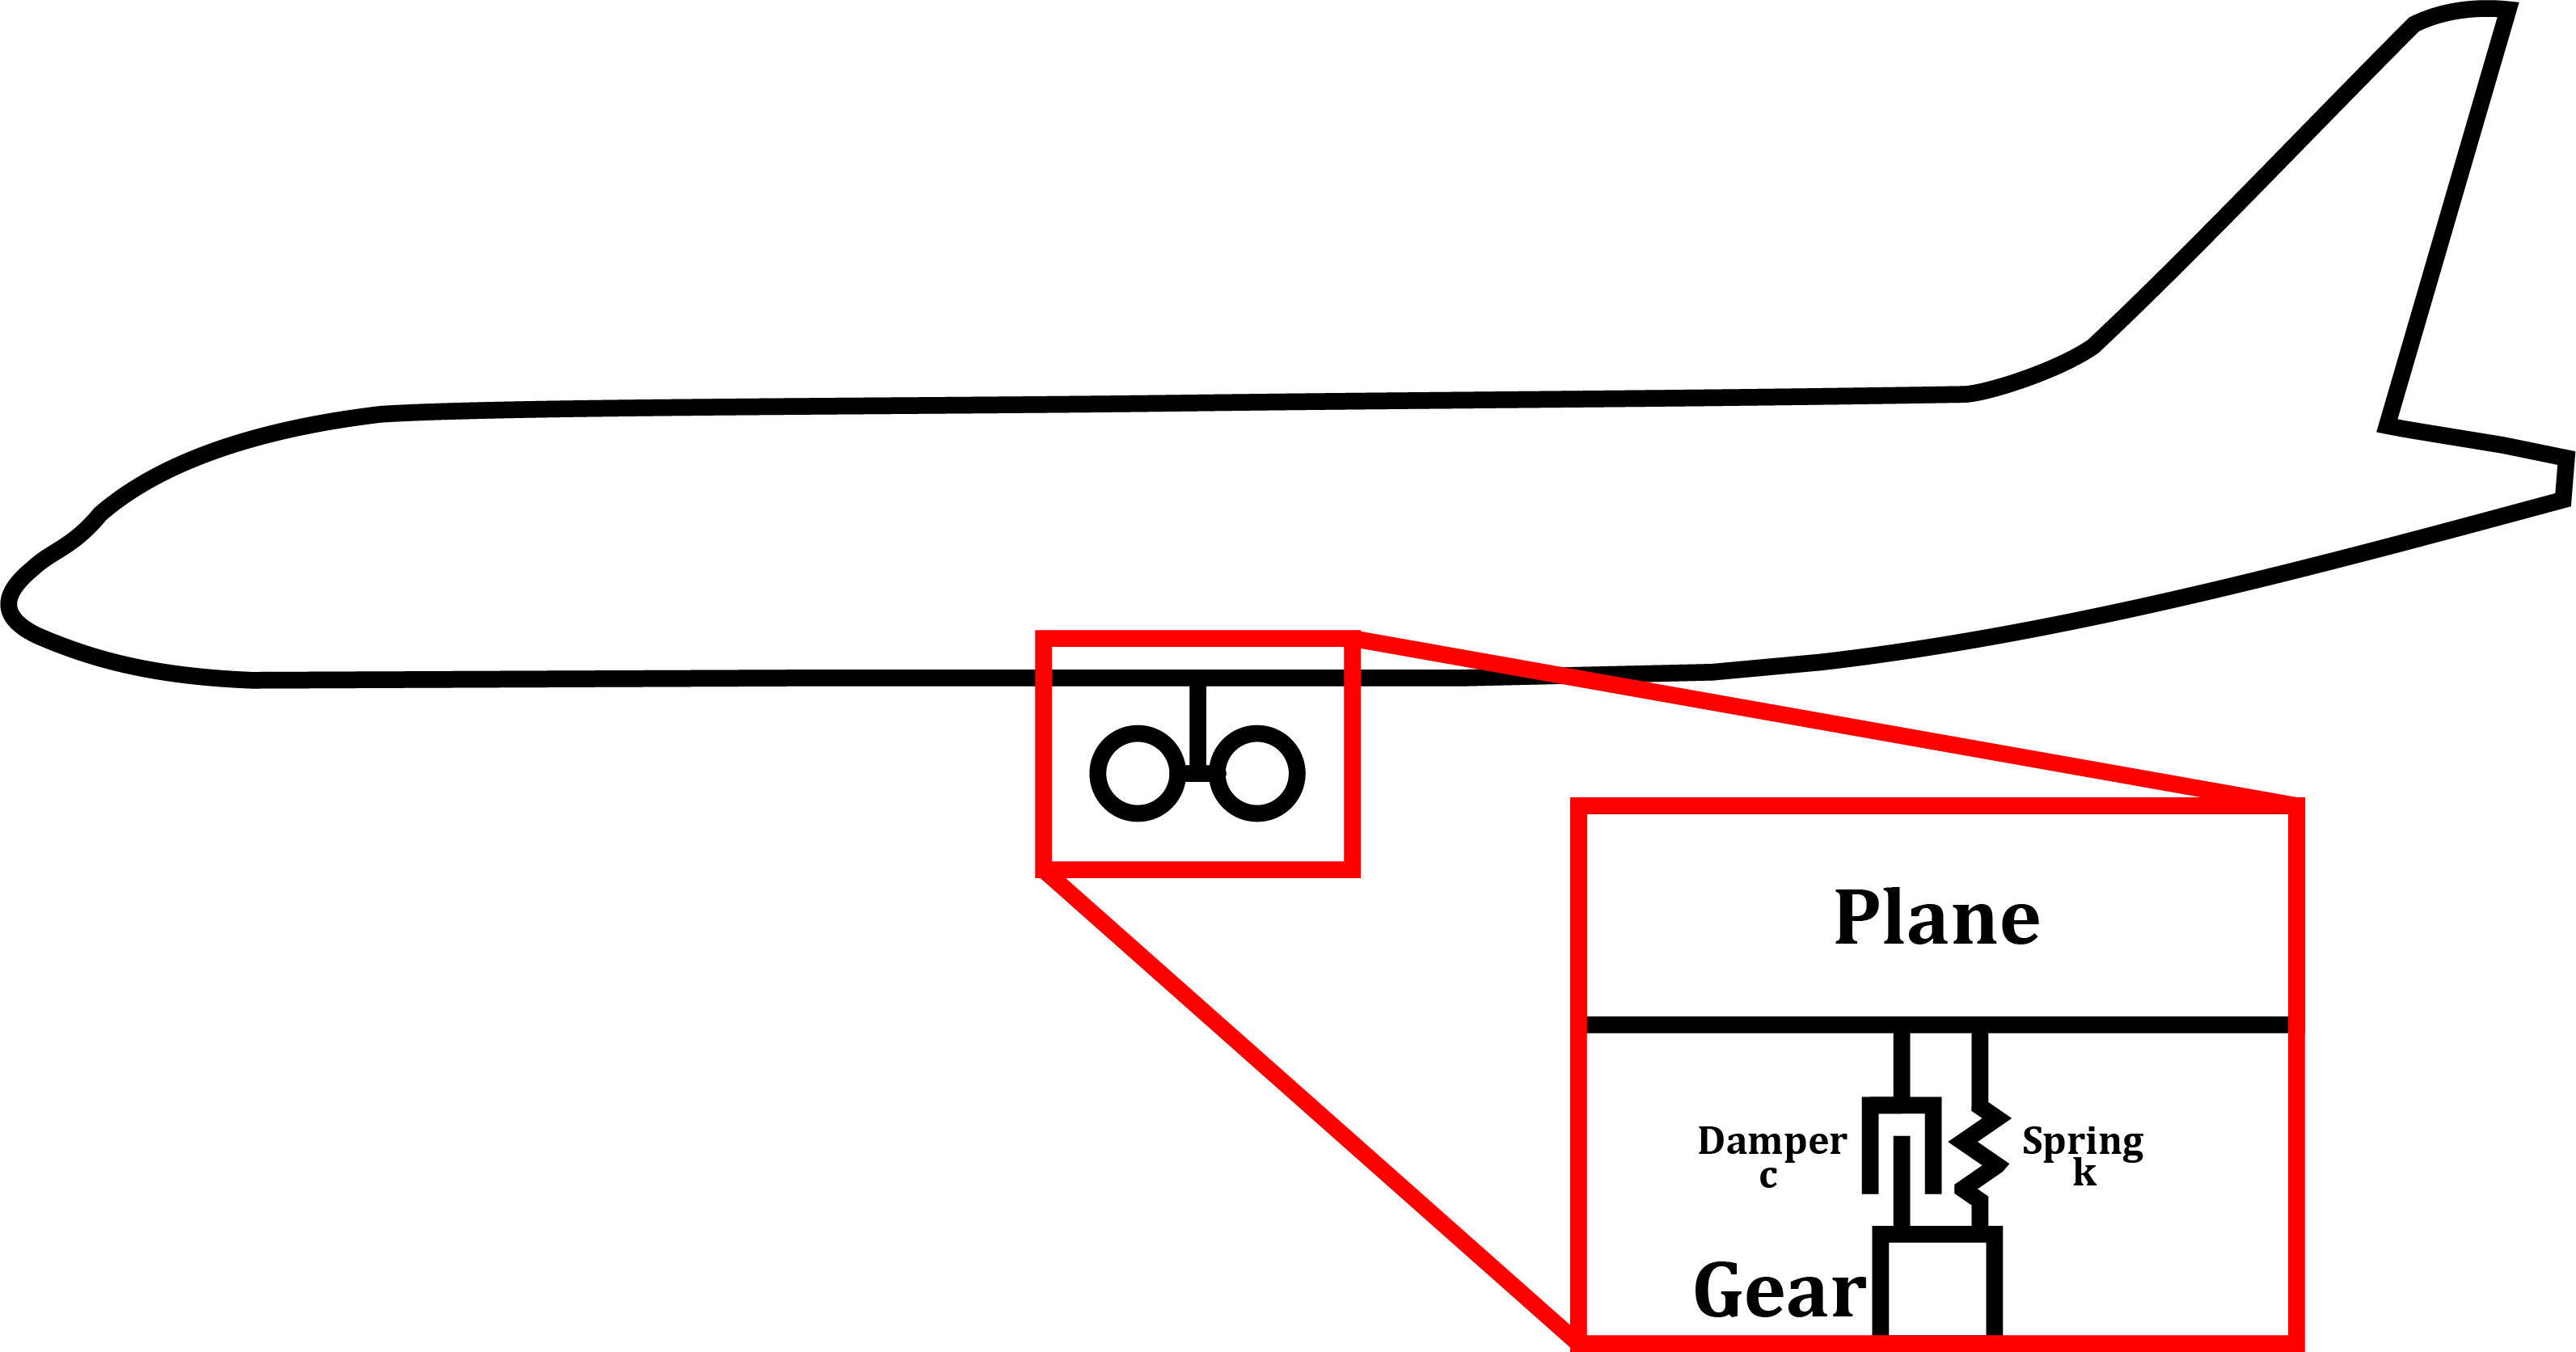
\includegraphics[width=0.6\textwidth]{FBD.png}
    \caption{Free Body Diagram}
    \label{fig:FBD}
\end{figure}

\begin{figure}[h!]
    \centering
    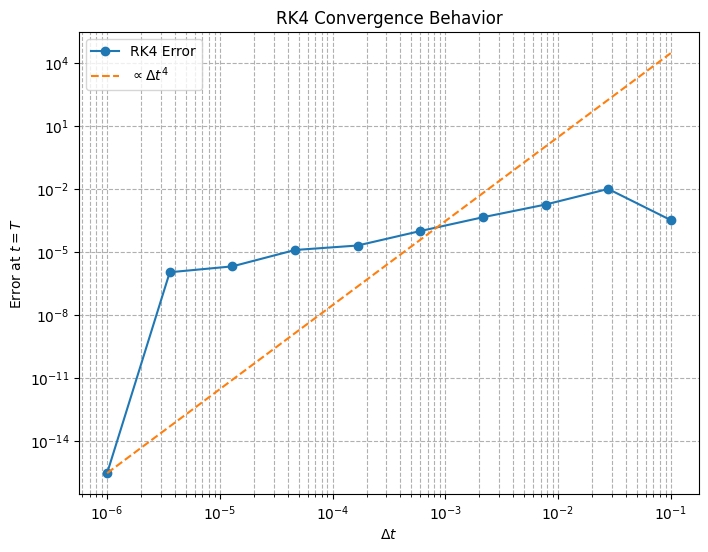
\includegraphics[width=0.6\textwidth]{RK4 Error.png}
    \caption{Error convergence analysis for different time steps.}
\end{figure}

\begin{figure}[h!]
    \centering
    \includegraphics[width=0.6\textwidth]{download.png}
    \caption{Effect of Time Step Size on Vertical Displacement z(t).}
\end{figure}

\begin{figure}[h!]
    \centering
    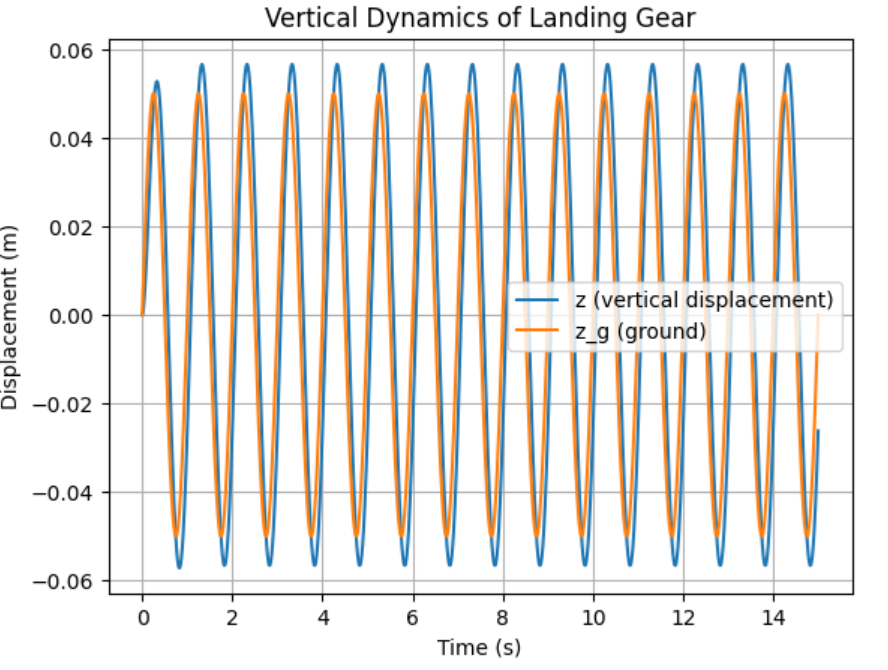
\includegraphics[width=0.6\textwidth]{c=6000.png}
    \caption{Vertical displacement of aircraft and ground, c=6000}
    \label{fig:c=6000}
\end{figure}

\begin{figure}[h!]
    \centering
    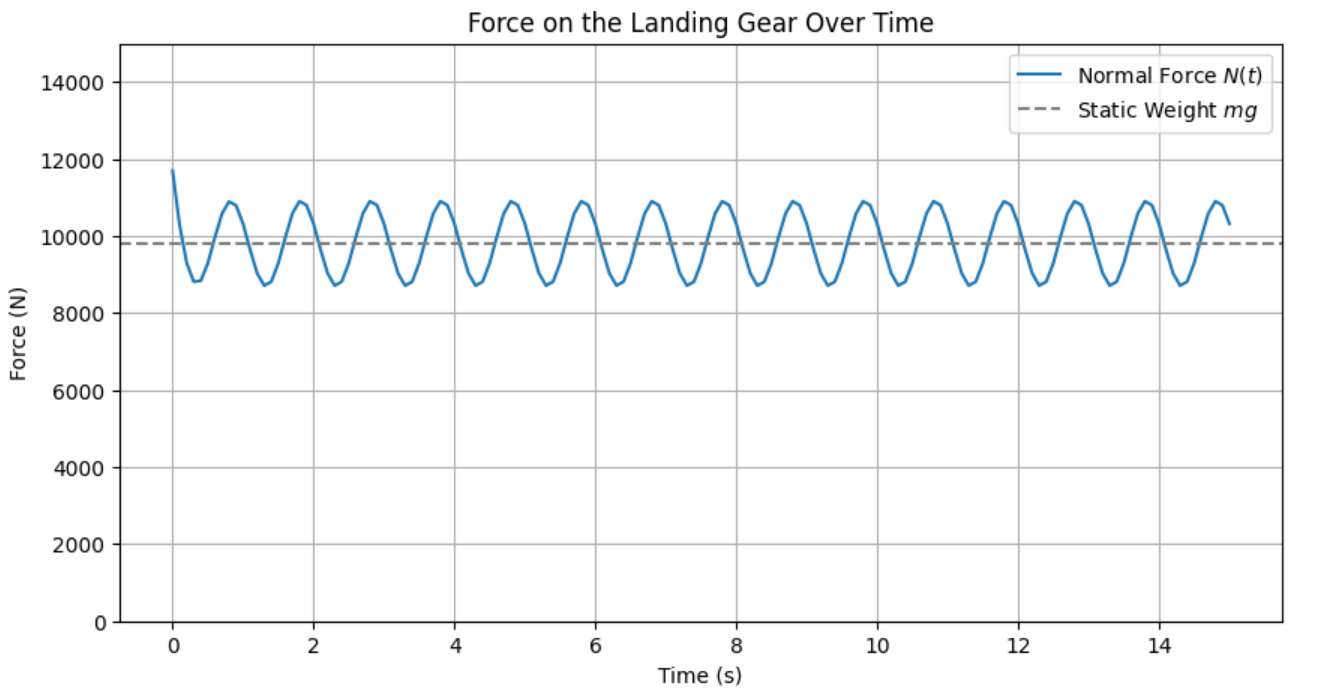
\includegraphics[width=0.6\textwidth]{force c=6000.png}
    \caption{Normal force on the aircraft from the ground, c=6000}
    \label{fig:force}
\end{figure}

\begin{figure}[h!]
    \centering
    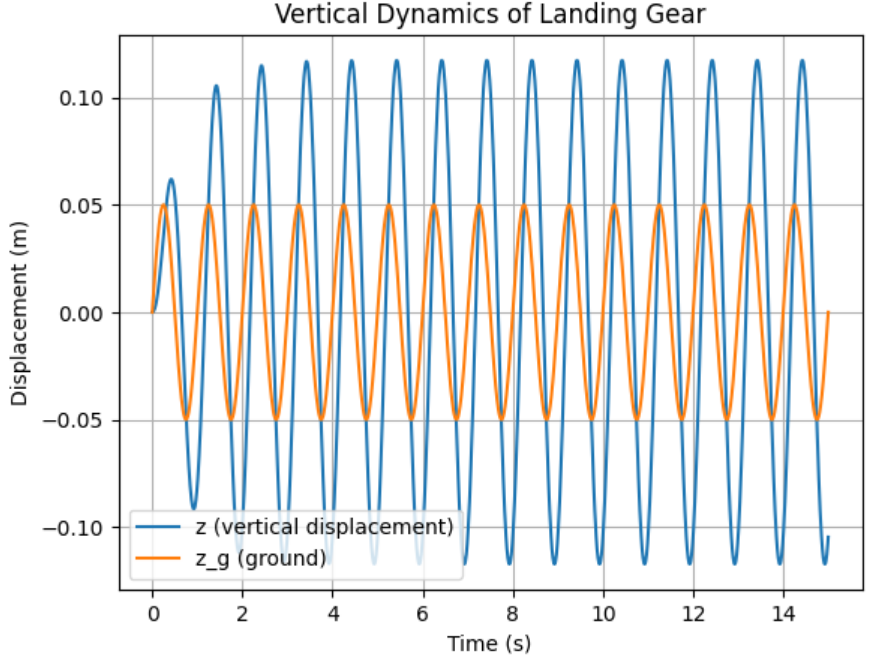
\includegraphics[width=0.6\textwidth]{c=1500.png}
    \caption{Vertical displacement of aircraft and ground, c=1500}
    \label{fig:c=1500}
\end{figure}

\begin{figure}[h!]
    \centering
    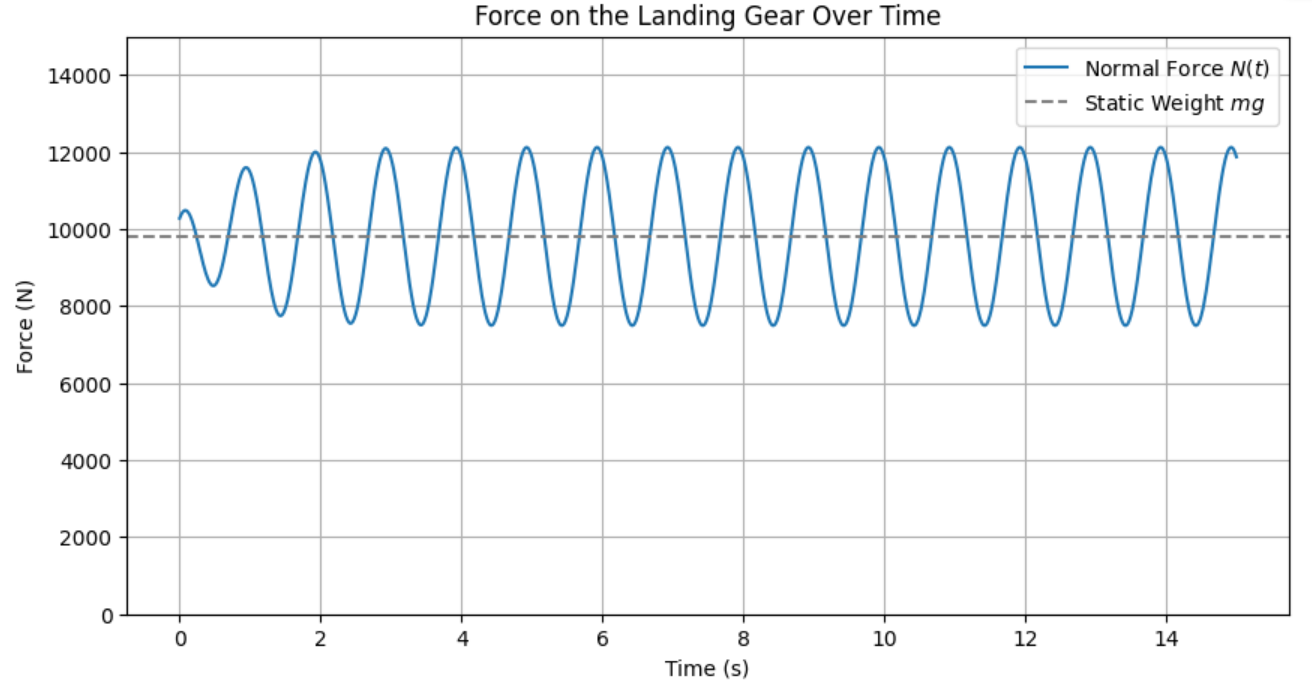
\includegraphics[width=0.6\textwidth]{force c=1500.png}
    \caption{Normal force on the aircraft from the ground, c=1500}
    \label{fig:force2}
\end{figure}

\begin{figure}[h!]
    \centering
    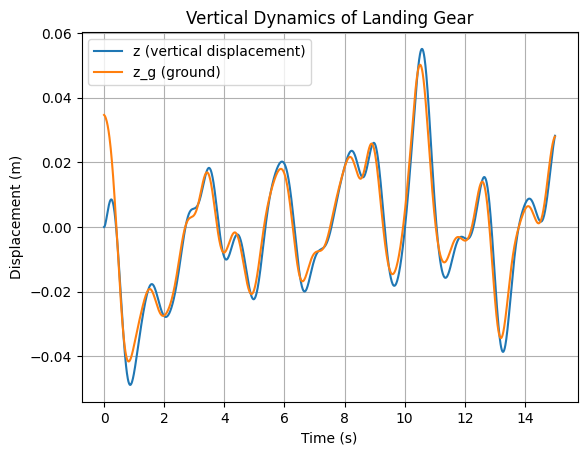
\includegraphics[width=0.6\textwidth]{RealGround.png}
    \caption{Vertical displacement of aircraft and ground, c=6000}
    \label{fig:RealGround}
\end{figure}

\begin{figure}[h!]
    \centering
    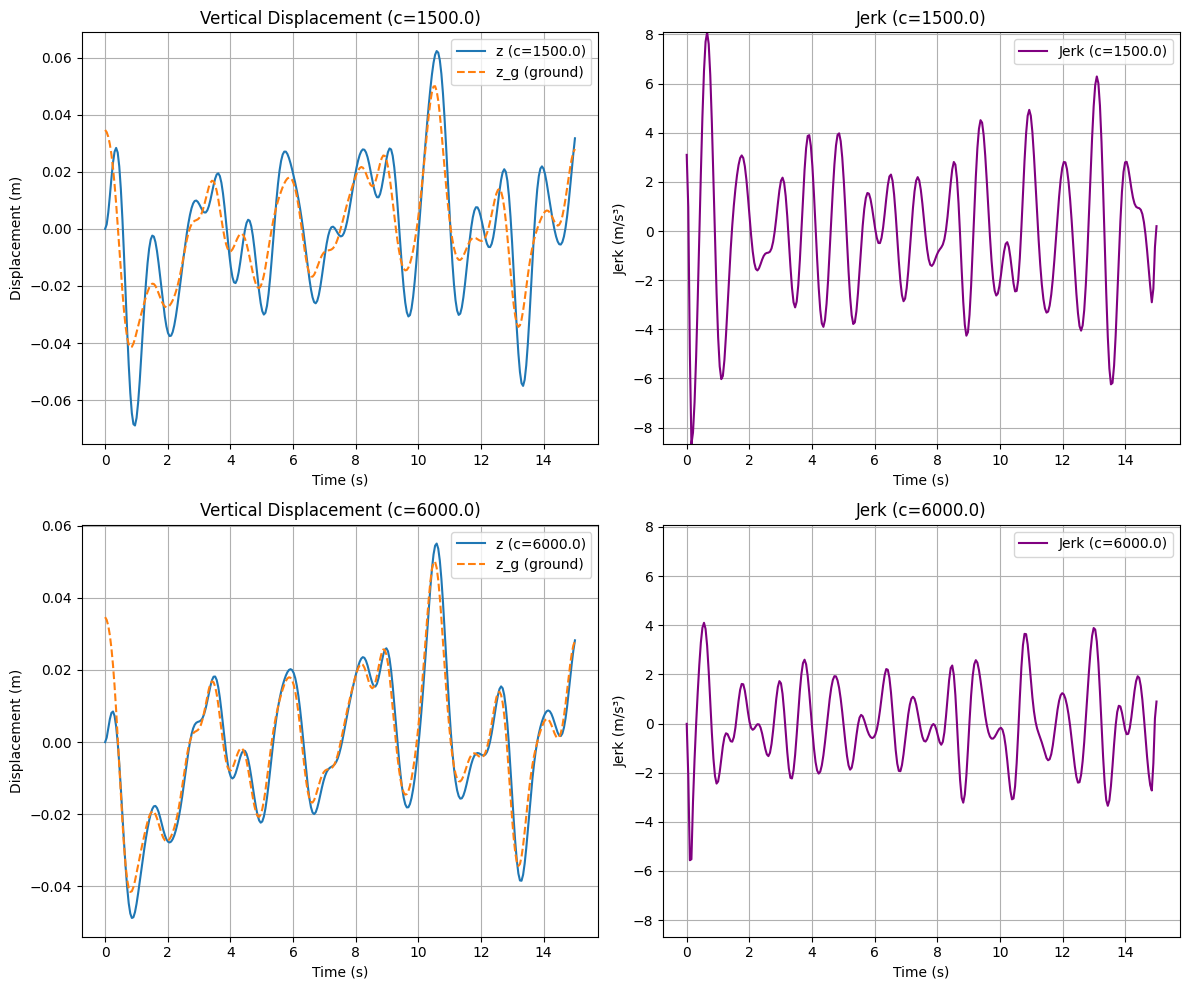
\includegraphics[width=0.8\textwidth]{Jerk.png}
    \caption{Jerk graphs for c=1500 and c=6000}
    \label{fig:Jerk}
\end{figure}

\end{questions}
\FloatBarrier

\section{Conclusion}
This project analyzed the coupled mass-spring-damper system for landing gear shock absorption. We formulated the equations of motion, implemented a numerical solver, and conducted simulations to study the effects of damping.

\subsection{Key Findings}
\begin{itemize}
    \item Higher damping reduces oscillations and experienced passenger jerk, but increases initial impact forces.
    \item The optimal damping ratio balances \textbf{impact force minimization} and \textbf{settling time reduction}.
    \item The RK4 method provided stable and accurate results even with complex ground profiles.
\end{itemize}

\subsection{Future Work}
Future extensions of this study could include:
\begin{itemize}
    \item Incorporating nonlinear damping effects.
    \item Modeling three-dimensional landing gear behavior.
    \item Experimentally validating the numerical results.
\end{itemize}

\textbf{Overall, this study provides valuable insights into landing gear design for improved shock absorption.}

\newpage

\section*{Acknowledgements}

We would like to thank Professor Goza and the AE370 course staff for designing such a thoughtful and engaging project. Working through the modeling, simulation, and validation steps helped us build a much deeper understanding of how numerical methods are applied to real engineering problems.

We also appreciate the help from the TAs throughout the semester whether it was answering questions during office hours, offering feedback on our progress, or helping us debug tricky edge cases, their support made a big difference.

Finally, we want to acknowledge our use of ChatGPT as a tool to support this project. We used it responsibly to:
\begin{itemize}
    \item Polish up LaTeX formatting and structure,
    \item Explore convergence testing strategies and simulation parameters,
    \item Double-check our understanding of certain numerical behaviors,
    \item Improve clarity in figure captions and write-up sections.
\end{itemize}

All the code, math, and written content in this report was created by us. ChatGPT was used like we’d use a textbook, Stack Overflow, or documentation, as a reference to help us work more effectively, not to replace our own understanding. We made sure everything aligns with the academic integrity policies at the University of Illinois.


\end{document}
